\documentclass[final,nocolorBG,a4,marieke,nototal,ps, accumulate,slideColor]{prosper}

\addtolength{\textheight}{-1cm}

\usepackage{pstricks,pst-node,pst-text,pst-3d}
\usepackage{amsmath}
\usepackage{alltt}
\usepackage{epsfig}

\usepackage{colordvi}
\usepackage{proof}
\usepackage{epsf}
\usepackage{amssymb}

\input{prooftree}
\newcommand{\textttbf}[1]{\texttt{\textbf{#1}}}
 \def \bsl       {\symbol{92}}
 \def \unsc      {\symbol{95}}

\title{Enforcing high-level security properties using JML}
\subtitle{}
\author{Marieke Huisman}
\institution{INRIA Sophia Antipolis
\medskip\\
\Blue{joint work with Mariela Pavlova, Gilles Barthe, Lilian Burdy \\Jean-Louis Lanet \& Igor Siveroni}}
\email{Marieke.Huisman@inria.fr}

\slideCaption{Security properties and JML}
\Logo{}
\begin{document} 

\maketitle

\overlays{2}{
\begin{slide}{Challenges within GECCOO}
\begin{itemize}
\item Formally specifying high-level security properties
\item Semantics of specifications
\item Composing specifications
\end{itemize}

\FromSlide{2}
\Blue{This talk: focus on first point}
\end{slide}
}

\begin{slide}{Contents}
\begin{itemize}
\item JML: what is there already
\item Security properties
\item A method for annotation generation
\item Towards security automata
\end{itemize}
\end{slide}
%\begin{slide}{Purpose of this talk}
%\begin{itemize}
%\item What is JML?
%\item Tools for JML
%\item JML and security properties
%  \begin{itemize}
%    \item What are security properties?
%    \item Limitations of JML
%    \item Our approach
%  \end{itemize}
%\item The future
%\end{itemize}
%\end{slide}

%\begin{slide}{Java Modeling Language}
%\begin{itemize}
%\item Behavioural interface specification language
%\item Developed by Gary Leavens \emph{et al.} at Iowa State University
%\item Annotations written as comments in source code
%\item The web-page: \Blue{\textttbf{\textbf{http://www.jmlspecs.org}}}
%\item Mailing list: \textttbf{jmlspecs-interest@lists.sourceforge.net}.
%\end{itemize}
%\end{slide}

\overlays{2}{
\begin{slide}{Design goals JML}
\begin{itemize}
\item Readable specifications
\item Provides unambiguous documentation
\item Usable for any Java application
\item Rigorous, formal semantics~-~amenable to tool support 
\\\FromSlide{2}{\Red{jmlc, ESC/Java(2), LOOP, Krakatoa, JACK}}
\end{itemize}
\end{slide}
}

%\begin{slide}{Method Specifications}
%\begin{itemize}
%\item Precondition
%\item Postcondition
%\item Exceptional postcondition
%\item Modifiable clause
%\end{itemize}
%\noindent Generic method specification:
%\begin{tabbing}
%ddd\=ddd\=ddd\=ddd\=ddd\= \kill 
%\>\Blue{\textttbf{/*@ public behavior}}\\
%\>\>\>\Blue{\textttbf{requires P;}}\\
%\>\>\>\Blue{\textttbf{modifies M;}}\\
%\>\>\>\Blue{\textttbf{ensures Q;}}\\
%\>\>\>\Blue{\textttbf{signals (e) R;}}\\
%\>\Blue{\textttbf{*/}} 
%\end{tabbing} 
%\end{slide}

%\begin{slide}{Example}
%\vspace*{-1em}
%{\small{\begin{alltt}
%\textbf{\Blue{/*@ behavior
%  @ modifies decimal;
%  @  ensures decimal == v * PRECISION;
%  @  signals (DecimalException e)
%  @          v < 0 && decimal == \bsl{}old(decimal);
%  @*/}
%public Decimal setValue(short v) 
%               throws DecimalException \{
%  if(v < 0) DecimalException.throwIt(
%                   DecimalException.OVERFLOW);
%  intPart = v; decPart = (short) 0;
%  return this; \}}
%\end{alltt}}}
%\end{slide}

%\overlays{3}{
%\begin{slide}{Class specifications}
%\FromSlide{1}
%\begin{description}
%\item[Model:] model variables to specify abstractly internal state of object
%\newline \emph{e.g.} \Blue{\textttbf{BoundedThing}} has \Blue{\textttbf{size},
%\textttbf{MAX\unsc SIZE}}
%\item[Ghost:] abstract variable, with special assignment \Blue{\textttbf{set}}
%\FromSlide{2}
%\item[Invariant:] properties of all publicly reachable states
%of object \newline 
%\Blue{\textttbf{invariant 0<=size \&\&
%size<=MAX\unsc SIZE}}
%\FromSlide{3}
%\item[Constraint:] relates pre and post states of methods
%\newline 
%\Blue{\textttbf{constraint MAX\unsc SIZE ==
%\bsl old(MAX\unsc SIZE)}}

%\end{description}
%\end{slide}
%}

%\begin{slide}{Example}
%{\small \begin{alltt}
%\textbf{
%public static final short MAX_DECIMAL_NUMBER = 
%                          (short) 32767;
%public static final short PRECISION = 
%                          (short) 1000;

%\Blue{/*@ spec_public*/} private short intPart = 
%                          (short) 0;
%\Blue{/*@ spec_public*/} private short decPart = 
%                          (short) 0;
%}
%\end{alltt}}
%\end{slide}

%\begin{slide}{Example - continued}
%{\small \begin{alltt}
%\textbf{\Blue{/*@ invariant 0 <= intPart && 
%  @           intPart <= MAX_DECIMAL_NUMBER &&
%  @           0 <= decPart && 
%  @           decPart < PRECISION; 
%  @
%  @ model int decimal;
%  @ represents decimal <- 
%  @            intPart * PRECISION + decPart;
%  @ depends decimal <- intPart, decPart; 
%  @*/}
%}
%\end{alltt}}
%\end{slide}

%\begin{slide}{Special keywords}
%\begin{itemize}
%\item Result of method call \Blue{\bsl result}
%\item Value in pre-state of method \Blue{\bsl old(\(E\))}
%\item Ensure object is newly allocated \Blue{\bsl fresh(\(E\))}
%\item All reachable objects \Blue{\bsl reach(\(E\))}
%\item And many others
%\end{itemize}
%\end{slide}

%\begin{slide}{More advanced method specifications}
%\begin{itemize}
%\item \Blue{normal\unsc behavior}: a method must terminate
%\item \Blue{exceptional\unsc behavior}: a method must throw an exception
%\item \Blue{diverges}: when a method may not terminate
%\item \Blue{measured\unsc by}: show termination of recursive functions
%\item \Blue{when}: for concurrency
%\end{itemize}
%Some of these possibilities better understood than others, still under development 
%\end{slide}

%\begin{slide}{Tools for JML}
%\begin{itemize}
%\item Various tools use JML as specification language
%\item Vary in precision and efficiency
%\item Range of tools: \Blue{run-time verification} - \Blue{static
%checking} - \Blue{interactive verification}
%\item Experiments show: balanced use of these tools increases
%productivity of application developers   
%\item Other approach: \\
% \Blue{Daikon} - detection of class invariants
%\end{itemize}
%\end{slide}

%\begin{slide}{Run-time verification: JMLC and Jass}
%\begin{itemize}
%\item JMLC: Iowa State University,\\ Jass: Univ. of Oldenburg
%\item Based on ideas Eiffel
%\item Assertions translated into \Blue{executable code}
%\item Basically: precondition tested when entering method,
%postcondition when leaving method
%\item Exception thrown when assertion violated
%\item \Blue{Extended testing}
%\item In addition: Jass accepts \Blue{trace-assertions}
%\end{itemize}
%\end{slide}

%\begin{slide}{Static checking: ESC/Java}
%\begin{itemize}
%\item Originally: Compaq, \\
%      ESC/Java2: Joe Kiniry/David Cok
%\item Compromise between \Blue{soundness/completeness} and \Blue{efficiency}
%\item Goal: efficiently finding common programming errors
%  \begin{itemize}
%     \item Nullpointer dereferencing
%     \item Indexing an array out of bounds
%  \end{itemize}
%\item Generation of proof obligations, proven with \Blue{Simplify}
%\item Used in several smart card application case studies 
%\end{itemize}
%\end{slide}


%\overlays{2}{
%\begin{slide}{Interactive verification: LOOP/Jive/Krakatoa}
%\begin{itemize}
%\item LOOP: Univ. of Nijmegen,\\ Jive: Univ. of Kaiserslautern,\\
%Krakatoa: LogiCal
%\item Interactive theorem prover for verification of proof obligations
%\item \Blue{Embedding in logic} theorem prover (LOOP) or
%\Blue{external generation} of proof obligations (Jive/Krakatoa)
%\item \Blue{High precision}, but...
%\FromSlide{2}
%\item \Blue{Labour intensive}
%\end{itemize}
%\end{slide}
%}

%\overlays{2}{
%\begin{slide}{Jack: a tool for engineers}
%\begin{itemize}
%\item Design goals:
%  \begin{itemize}
%     \item High correctness assurance
%     \item Accessible user interface 
%     \item Prover independence
%     \item High degree of automation
%  \end{itemize}
%\FromSlide{2}
%\item Consequences:
%  \begin{itemize}
%     \item Developed as plug-in IDE Eclipse
%     \item Connections with automatic provers (B prover, Simplify, HarVey, 
%           \ldots) 
%  \end{itemize}
%\end{itemize}
%\end{slide}
%}

\overlays{2}{
\begin{slide}{Limitations of JML}
\begin{itemize}
  \item Specifications restricted to a \Blue{single class}
  \item Specifications restricted to \Blue{functional behaviour}
  \item Not much support for refinement 
\end{itemize}
\FromSlide{2} In order to verify security properties, one needs to
overcome these limitations
\end{slide}
}

\begin{slide}{Enforcing security properties}
\begin{itemize}
\item \Blue{Security expert}: from global notions of security to set
of rules
\item \Blue{Developers}: try to obey rules
\item \Blue{Security audit}: manual code inspection whether rules
obeyed
\item Need for tools to help security audit
\end{itemize}
\end{slide}

\overlays{3}{
\begin{slide}{Questions to be addressed}
\begin{itemize}
\item Relation between security notions and rules
\onlySlide{1}{\item Guaranteeing rules are obeyed}\vspace*{-1.5em} 
\FromSlide{2}\item \Red{Guaranteeing rules are obeyed}
\FromSlide{3}\item Extension towards security automata: \emph{bridging} the gap
between security notions and rules
\end{itemize}
\end{slide}
}

\overlays{5}{
\begin{slide}{High-level security rules}
\begin{itemize}
  \item Atomicity
  \onlySlide{1}{
  \item Applet life cycle
  \item Exception handling
  \item Access control}
  \onlySlide{2}{\vspace*{-4.5em}\begin{itemize}
                     \item No nested transactions
                     \item No uncaught exception in transactions
                     \item Bounded retries authentication
                  \end{itemize}
  \item Applet life cycle
  \item Exception handling
  \item Access control}
  \fromSlide{3}{\vspace*{-8.5em}\item Applet life cycle}
  \onlySlide{3}{\begin{itemize}
                         \item Authenticated initialisation
                         \item Authenticated unblocking
                         \item Single personalisation
                \end{itemize}
  \item Exception handling
  \item Access control}
  \fromSlide{4}{\vspace*{-7em}\item Exception handling}
  \onlySlide{4}{\begin{itemize} 
                   \item Only ISOExceptions at top-level
                \end{itemize}
  \item Access control}
  \fromSlide{5}{\vspace*{-3em}
  \item Access control
          \begin{itemize}
             \item Only selectable applications shareable
          \end{itemize}
  }
\end{itemize}
\end{slide}
}

\begin{slide}{Architecture}
 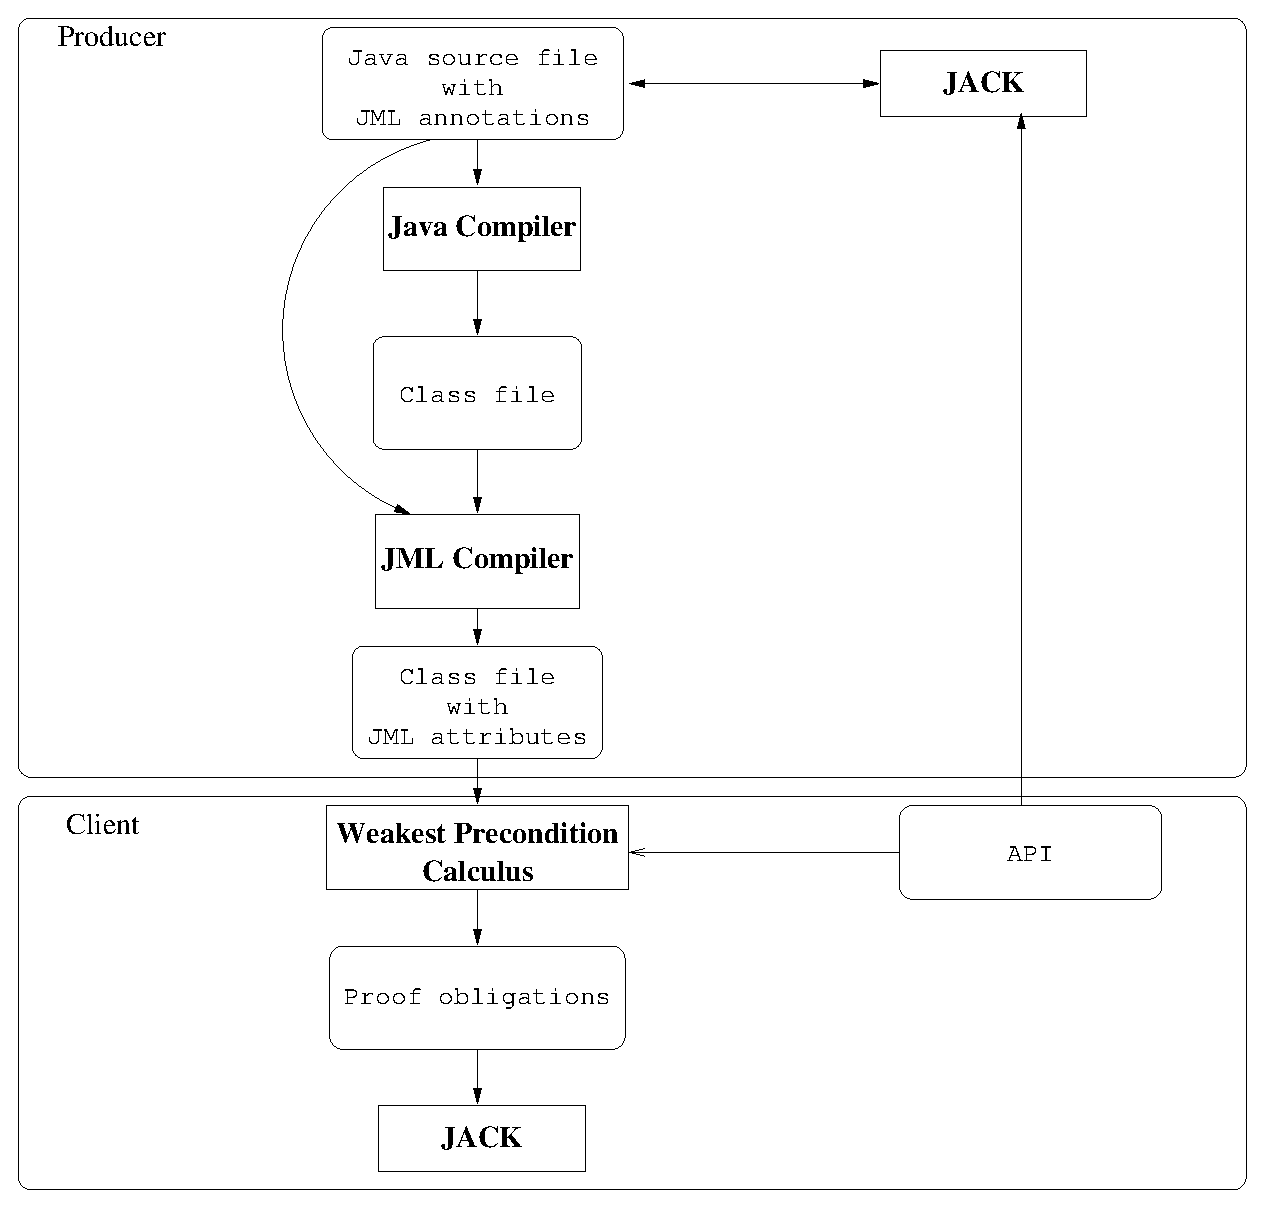
\psfig{file=../Papers/isaac/architecture.eps,width=\textwidth}
\end{slide}

\begin{slide}{Assertion generation}
Two phases:
\begin{itemize}
\item \Blue{synthesising} core-annotations
\item \Blue{weaving} annotations throughout the application
\end{itemize}
\ \smallskip\\
\Blue{Synthesising}: for each property annotations have to be defined
\bigskip\\
\Blue{Weaving}: algorithm for pre- and postcondition generation
\end{slide}

\begin{slide}{Example core-annotations}
\Red{No nested transactions}
\begin{alltt}
\Blue{\textbf{/*@ static ghost int TRANSACT == 0; @*/}}
\end{alltt}
\ \smallskip\\
Method \textttbf{beginTransaction}
\begin{alltt}
\Blue{\textbf{/*@ requires TRANSACT == 0;
  @ assignable TRANSACT;
  @ ensures TRANSACT == 1; @*/}}
\textbf{public static native 
   void beginTransaction() 
        throws TransactionException;}
\end{alltt}
\ \smallskip\\
Similar annotations for \textttbf{commitTransaction},
\textttbf{abortTransaction} 
\end{slide}


\begin{slide}{Preconditions for methods}
\begin{alltt}
\textbf{public void m() \{
   ...
   \Blue{// will require TRANSACT == 0}
   JCSystem.beginTransaction();
   \Blue{// TRANSACT modified, ensures TRANSACT == 1}
   ...
   \Blue{// will require TRANSACT == 1}
   JSSystem.commitTransaction();
   \Blue{// TRANSACT modified, ensures TRANSACT == 0}
   ...
   \}}
\end{alltt}
\end{slide}

\begin{slide}{Preconditions for methods}
\begin{alltt}
\textbf{public void m() \{
   ...
   \Blue{// will require TRANSACT == 0}
   JCSystem.beginTransaction();
   \Blue{// TRANSACT modified, ensures TRANSACT == 1}
   ...
   \Blue{// will require TRANSACT == 1}
   JSSystem.commitTransaction();
   \Blue{// TRANSACT modified, ensures TRANSACT == 0}
   ...
   \}}
\end{alltt}
\ \smallskip\\
\Blue{Thus: precondition for \texttt{m()}: \texttt{TRANSACT
== 0}}
\end{slide}

\begin{slide}{Some assumptions we make}
\begin{itemize}
  \item Only variables in annotations are static and ghost of primitive type
  \item Appropriate modelling of programs
  \item Existence of function {\large\textsf{\Red{mod}}}: set of static ghost
variables modified by statement 
\end{itemize}
\end{slide}

\begin{slide}{Algorithm for precondition generation}
\begin{itemize}
   \item \Blue{Method declaration}
\[\mathsf{\PineGreen{pre}}(m)  =  \mathsf{\PineGreen{pre}}(\mathsf{body}(m), \emptyset)\]
   \item \Blue{Composition}
\[\mathsf{\PineGreen{pre}}(s_1 \mathtt{;} s_2, V)  =  \mathsf{\PineGreen{pre}}(s_1, V) \cup 
                                          \mathsf{\PineGreen{pre}}(s_2, V \cup
\mathsf{\Red{mod}}(s1))\]
   \item \Blue{Method call}
\[\mathsf{\PineGreen{pre}}(\mathsf{\Blue{call}}(n),V)  =  
                \{ p \mid p \in \mathsf{\PineGreen{pre}}(n) \wedge 
                          \mathsf{fv}(p) \cap V = \emptyset\}\]
\end{itemize}
\end{slide}

\begin{slide}{Algorithm for precondition generation - branching statements}
\begin{itemize}
   \item \Blue{Conditional}
\[
\mathsf{\PineGreen{pre}}(\mathtt{if\:(} c \mathtt{)\:} s_1 \mathtt{\:else\:} s_2,
V)  = 
\begin{array}[t]{l}
   \mathsf{\PineGreen{pre}}(c, V) \:\cup \\
   \mathsf{\PineGreen{pre}}(s_1, V \cup \mathsf{\Red{mod}}(c)) \:\cup\\
   \mathsf{\PineGreen{pre}}(s_2, V \cup \mathsf{\Red{mod}}(c))
\end{array}\]
\item \Blue{Try catch}
\[\mathsf{\PineGreen{pre}}(\mathtt{try\:} s_1 \mathtt{\:catch\:(} E \mathtt{)\:} s_2, V)  =  \begin{array}[t]{l}
   \mathsf{\PineGreen{pre}}(s_1, V) \:\cup \\
   \mathsf{\PineGreen{pre}}(s_2, V \cup \mathsf{\Red{mod}}(s1))
  \end{array}\]
\end{itemize}
\end{slide}




\begin{slide}{Experiments: checking atomicity properties}

\Red{No uncaught exceptions in transactions}\smallskip\\

\begin{alltt}
\textbf{\Blue{/*@ exsures (Exception) TRANSACT == 0; @*/}
public static native void 
   commitTransaction() 
         throws TransactionException;}
\end{alltt}
Annotation propagated to each statement block, ending with commit.
\end{slide}

\begin{slide}{Experiments: checking atomicity properties}
\Red{No pin-verification within transaction}\smallskip\\

\begin{alltt}
\textbf{\Blue{/*@ requires TRANSACT == 0; @*/}
public boolean check(byte[] pin, 
                     short offset, 
                     byte length);}
\end{alltt}
\end{slide}

\begin{slide}{Results}
\begin{itemize}
\item Tested on several realistic smart card applications
\item One core-annotation can give rise to many annotations in
different classes (26 annotations, spread over 5 different classes)
\item Several violations found: uncaught exceptions possible within
transactions 
\end{itemize}
\end{slide}

\begin{slide}{Uncaught exception within transaction}
\begin{alltt}
\textbf{void appExchangeCurrency(...) \{
   ...
   \Blue{/*@ exsures (Exception) TRANSACT == 0; @*/} \{
      ...
      JCSystem.beginTransaction();	
      try \{balance.setValue(decimal2);
            ...
      \} catch (DecimalException e) \{
         ISOException.throwIt(
              PurseApplet.OVERFLOW);
      \}
      JCSystem.commitTransaction();
   \}
   ...\}}
\end{alltt}
\end{slide}


\begin{slide}{Towards more generality:\\ Security automata}
\begin{itemize}
\item \Blue{Security automaton}: monitors program behaviour,
blocking/error upon unwanted behaviour 
\item Use security automata to express security properties
\item Automatic generation of core-annotations
\item Use any JML tool to check whether program respects the property
\end{itemize}
\end{slide}

\overlays{2}{
\begin{slide}{Correctness}
\begin{center}
\Blue{If program satisfies annotations \\
      then it respects the security property}
\end{center}
\ \smallskip\\
\FromSlide{2}
Igor Siveroni (post doc) works on this\\
First proof for simple while-language on the way
\end{slide}
}

\overlays{3}{
\begin{slide}{If program satisfies annotations \\
      then it respects the security property}
Approach:
\begin{itemize}
\item If program satisfies annotations, run-time monitoring (with
\texttt{jmlc}) will never block  \Blue{(known result)}
\FromSlide{2}\item If run-time monitoring (with \texttt{jmlc}) of annotated program
never blocks, security automaton never blocks\\
\Blue{true for core-annotations, preserved by each propagation step}
\FromSlide{3}\item If security automaton does not block, program respects the
security property \Blue{(known result)}
\end{itemize}
\end{slide}
}


\begin{slide}{Future issues}
\begin{itemize}
\item Other formalisms to express security properties (with
translation into JML)?
\item Translations into other formalisms
\item Do we need liveness?
\end{itemize}
\end{slide}

\begin{slide}{Theoretical foundations: abstract weakest precondition}
Abstract wp-calculus \PineGreen{\(\mathsf{wp}^\#\)}: considers only static 
ghost variables\\
Example rules:
\[
\begin{array}{l}
\mathsf{\PineGreen{wp}}^{\PineGreen{\#}}(\mathtt{if
(}c\mathtt{)}s_1\mathtt{\:else\:}s_2,Q) =\\
\qquad
\mathsf{\PineGreen{wp}}^{\PineGreen{\#}}(c, \mathsf{\PineGreen{wp}}^{\PineGreen{\#}}(s_1, Q)) \wedge
\mathsf{\PineGreen{wp}}^{\PineGreen{\#}}(c,
\mathsf{\PineGreen{wp}}^{\PineGreen{\#}}(s_2, Q))
\end{array}
\]

\[
\mathsf{\PineGreen{wp}}^{\PineGreen{\#}}(\mathsf{\Blue{call}}(m), Q) =
  \mathsf{\Blue{requires}}(m) \wedge 
  \forall \mathsf{\Red{mod}}(m). (\mathsf{\Blue{ensures}}(m) \Rightarrow Q)
\]
\end{slide}

\begin{slide}{Results}
\begin{itemize}
\item Any proof in abstract wp-calculus, is proof in standard
wp-calculus
\[
\forall P, Q\colon\mathsf{Pred}, s\colon\mathsf{Stmt}. 
(P \Rightarrow \mathsf{\PineGreen{wp}}^{\PineGreen{\#}}(s, Q)) \Rightarrow
               (P \Rightarrow \mathsf{\PineGreen{wp}}(s, Q))
\]
\item Precondition generation computes the \emph{free} part of the
abstract weakest precondition
\[
\exists F\colon\mathsf{Pred}.  
             \mathsf{\PineGreen{wp}}^{\PineGreen{\#}}(s, \lambda x. \mathsf{true}) = 
             (\mathsf{\PineGreen{pre}}(s, \emptyset) \wedge \forall
              \mathsf{\Red{mod}}(s). F) 
\]
\end{itemize}
\end{slide}

\end{document}